% DOC SETTINGS ===================================
\documentclass{article}
\usepackage[utf8]{inputenc}
\usepackage{fancyhdr}
\pagestyle{fancy}
\usepackage{geometry}
 \geometry{
 a4paper,
 total={170mm,257mm},
 left=20mm,
 top=25mm,
 }
\fancyheadoffset{0mm}
\lhead{ECE3504 HW2}
\rhead{Kavin Thirukonda 2021}
\usepackage{steinmetz}
\usepackage{listings}
\usepackage{circuitikz}
\usepackage{mathtools}  
\mathtoolsset{showonlyrefs} 
\cfoot{}
% DOC SETTINGS ===================================
\begin{document}
\section*{Problem 1 (6 points)}
Provide the MIPS core instructions(s) need to load the following 32-bit constants in to register \$t1.
\begin{enumerate}
    \item 0xFFFFFFF6
\begin{verbatim}
lui $t1, 1111 1111 1111 1111
ori $t1, 1111 1111 1111 0110
\end{verbatim}
    \item 0x00000268
\begin{verbatim}
li $t1, 0000 0010 0110 1000 
\end{verbatim}
    \item 0x12345678
\begin{verbatim}
lui $t1, 0001 0010 0011 0100 
ori $t1, 0101 0110 0111 1000
\end{verbatim}
\end{enumerate}
\section*{Problem 2 (6 points)}
Provide at least 3 distinct MIPS assembly language instructions to clear the contents of register \$s3.
\begin{verbatim}
sub $s3, $s3, $s3
\end{verbatim}
\begin{verbatim}
li $s3, 0
\end{verbatim}
\begin{verbatim}
andi $s3, $s3, 0
\end{verbatim}
\begin{center}
    Not quite sure if this is what the problem is asking for but thats what I interpreted I guess.
\end{center}
\section*{Problem 3 (10 points)}
The MIPS ISA has shift left logical (sll), shift right logical (srl) and shift right arithmetic (sra) instructions. Why is there no shift left arithmetic (sla) instruction?
\begin{center}
    Because they essentially do the same thing so having a different instruction for them is redundant and would add unnecessary hardware. Similar to how there is no NOT operation because there it can be replaced with NOR with ease.
\end{center}
\section*{Problem 4 (15 points)}
Provide a MIPS assembly language fragment to check if an address contained in register \$s0 is a multiple of 5. If this is the case then register \$s1 should be set to 1, and if this is not the case then register \$s1 should be set to 0.
\begin{verbatim}
.text
main:
    andi $s1, $s0, 4
    beq $s1, $zero, end
    li $s1, 1
end:
    li $v0, 10
    syscall
\end{verbatim}
\section*{Problem 5 (15 points)}
Provide a MIPS assembly language fragment to assign \$t0 to be the 32-bit NAND of the values in registers \$t1 and \$t2.
\begin{verbatim}
.text
main:
    and $t0, $t1, $t2
    nor $t0, $t0, $zero
    li $v0, 10
    syscall
\end{verbatim}
\newpage
\section*{Problem 6 (24 points)}
\begin{verbatim}
while(n > 1){
    if(n is even)
        n = n/2
    else
        n = 3 * n + 1
}
\end{verbatim}

\begin{verbatim}
.text
    ldi $t1, 1
main:
    ble $t3, $t1, end 
    andi $t0, $t3, 1
    beq $t0, $zero, mult  
    sra $t3, $t3, 1    
    jal main 
mult:
    lw $t0, $t3
    sll $t3, $t3, 1
    add $t3, $t3, $t0
    jal main
end:
    li $v0, 10
    syscall
\end{verbatim}
\section*{Problem 7 (24 points)}
\begin{verbatim}
Fib[0] = 0;
Fib[1] = 1;
for(i = 2; i < 100; i++){
    Fib[i] = Fib[i-1] + Fib[i-2];
}
\end{verbatim}
\begin{verbatim}
.text
    lui $s0, 0x1000
    sw $zero, 0($s0)
    addi $t0, $zero, 1
    sw $t0, 4($s0)
    li $t1, 2
main:
    bge $t1, 100, end 
    sll $t2, $t1, 2
    add $t2, $t2, $s0 
    addi $t3, $t2, -4
    lw $t3, 0($t3)
    addi $t4, $t2, -8
    lw $t4, 0($t4)
    addu $t3, $t3, $t4
    sw $t3, 0($t2)
    addi $t1, $t1, 1
    j main
end:
    li $v0, 10
    syscall
\end{verbatim}
\begin{center}
    \boxed{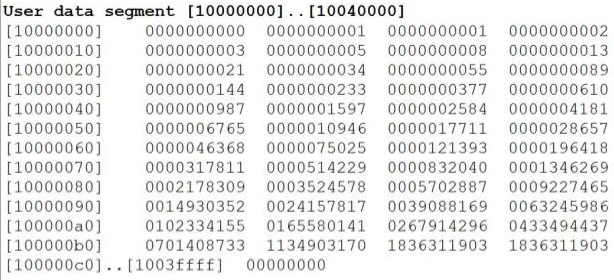
\includegraphics[width = .32\textwidth]{fib.png}}
\end{center}
\end{document}
